% !TEX root = ../thesis.tex

\chapter{Analytická časť}

This chapter covers analysis of genome structure of different organisms, or, in other words, biological background which is a necessity for creating any bioinformatics software.
Moreover, it particularly describes existing solutions for genome data representing. 
Each of the mentioned topics is described in the subsection corresponding to it.

\section{General Genome Structure}
In most eukaryotic and prokaryotic organisms the hereditary material is either linear double-stranded DNA (deoxyribonucleic acid) molecules or a circular double-stranded DNA molecule. 
However, some extracellular life forms, might use RNA (ribonucleic acid) as the building block for their genome. 
For instance, viruses have a genome composed of either single-stranded DNA, double-stranded DNA or RNA, depending on the type of a virus. 
Therefore, a genome itself, is the complete content of genetic information in an organism, or in other words, all the unique DNA (RNA) sequences the organism possesses. 

%%%%%%%%%%%%%%%%%%%%%%%%%%%%%%%%%%%%%%%%%%%%%%%%%%%%%%
\subsection{Nucleotides: the basic subunit of genome}
%%%%%%%%%%%%%%%%%%%%%%%%%%%%%%%%%%%%%%%%%%%%%%%%%%%%%%
Both of DNA and RNA  are polymeric molecules, that are composed of linear chains of various combinations of four different subunits, called nucleotides. 
The nucleotide itself is the basic unit of the DNA and RNA molecules, the monomer, which, however, could be found in the cell not only as the bearer of the genetic information, 
but also as a carrier of energy used to power enzymatic reactions \cite{AnalysisOfGenesAndGenomes}. 
A five-carbon-atom sugar, a phosphate group and a nitrogenous base are three distinct components which, combined together, make up the quite complex nucleotide molecule. 
The combination of sugar and base is called a nucleoside, while the phosphate-sugar-base is termed a nucleotide. 

\begin{figure}[!ht]
	\centering
	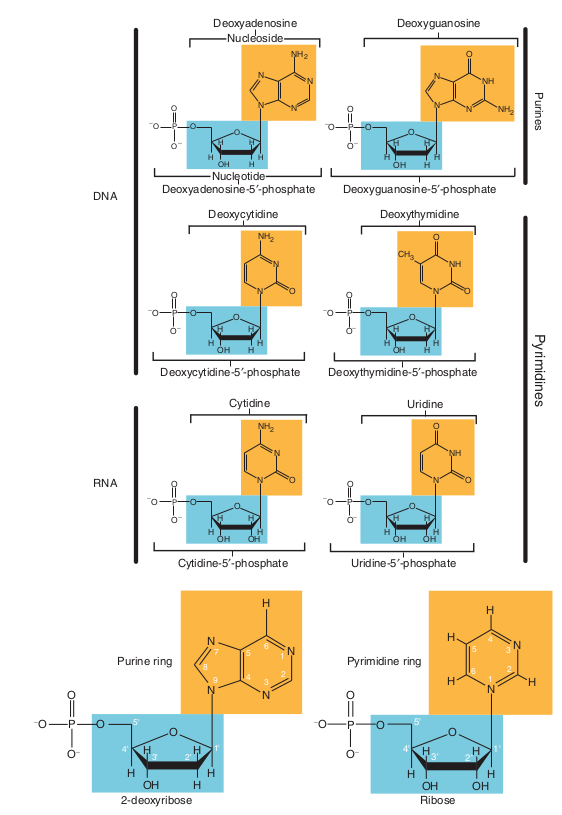
\includegraphics[width=.85\textwidth]{figures/bases}
	\caption{The structures of the pyrimidines and purines found in DNA and RNA. The sugar groups are highlighted in blue and the nitrogenous bases are highlighted in orange. 
	The atoms of the sugar are numbered from 1 to 5. The atoms of the purine ring are numbered from 1 to 9, 
	while those of the pyrimidine ring are numbered from 1 to 6. \label{o:nucleotide}}
\end{figure}

Dinucleotide, trinucleotide and polynucleotide are the terms corresponding to two, three or many nucleotides connected with each other respectively.

A nucleotide can be either a double-ringed purine or a single-ringed pyrimidine. 
Guanine (G) and adenine (A) are the common purines for both of DNA and RNA; the pyrimidine called cytosine (C) is also present in both nucleic acids. 
However, the pyrimidine uracil (U) is limited only to RNA, being replaced with thymine (T) in DNA. 
There are merely two base-pair combinations that are permissible – A base-paired with T (U) and C base-paired with G. 
It happens due to the geometries of the nucleotide bases and relative positions of atoms which participate in the connection \cite{MolecularGenetics}.
This property makes two sequences of polynucleotides in helix complement. 

\begin{figure}[!ht]
	\centering
	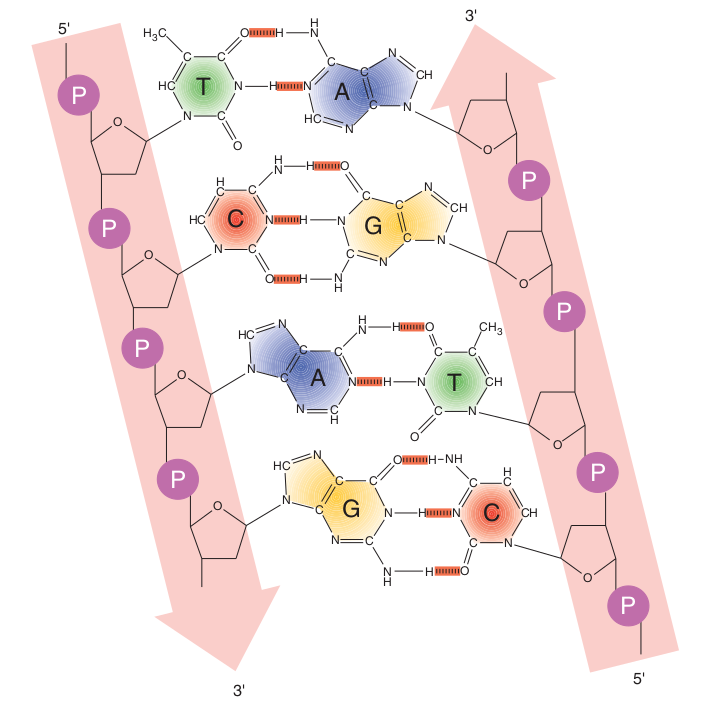
\includegraphics[width=.85\textwidth]{figures/nucleotides.png}
	\caption{DNA base pairing and complementation. The two chains of the helix, arrowed in the 5` to 3` direction, are antiparallel. The bases on one strand of the helix
	are complementary to those on the opposite strand, A always base pairs with T and G always base pairs with C \label{o:nucleotide}}
\end{figure}

Discrete nucleotides are attached to each other through sugar–phosphate bonds that connect the phosphate group on the 5’ carbon of one nucleotide with the hydroxyl group on the 3’ carbon of another nucleotide. 
The base pairing between adenine and thymine (uracil) involves two hydrogen bonds, while between cytosine and guanine involves three hydrogen bonds.

%%%%%%%%%%%%%%%%%%%%%%%%%%%%%%%%%%%%%%%%%%%%%
\subsection{Nucleodic acid spatial stucture}
%%%%%%%%%%%%%%%%%%%%%%%%%%%%%%%%%%%%%%%%%%%%%
As the three-dimensional structure of a nucleotide is not completely rigid, it is possible for DNA to have various spatial architectures: 
A-form, B-form, Z-form and the circular one. The position of the base relatively to the five-carbon-atom sugar can be changed by a rotation 
around the N-glycosidic bond and, in this way, significantly affect the three dimensional configuration of the molecule and helix consequently.

\begin{table}[!ht]
	\caption{DNA double helix}\label{t:1}
	\smallskip
	\centering
	
	\begin{tabular}{ |p{3cm}||p{3cm}|p{3cm}|p{3cm}|  }
		\hline
		\multicolumn{4}{|c|}{Features of the different conformations of the DNA double helix} \\
		\hline
		Feature& B-DNA & A-DNA & Z-DNA\\
		\hline
		\hline
		Type of helix & Right-handed & Right-handed & Left-handed\\
		\hline
		Number of base pairs per turn & 10 & 11 & 12\\
		\hline
		Distance between base pairs (nm) & 0.34 & 0.29 & 0.37\\
		\hline
		Distance per complete turn (nm) & 3.4 & 3.2 & 4.5\\
		\hline
		Diameter (nm) & 2.37 & 2.55 & 1.84\\
		\hline
		Major groove & Wide, deep & Narrow, deep & Flat\\
		\hline
		Minor groove & Narrow, shallow & Wide shallow & Narrow, deep\\
		\hline
	\end{tabular}
\end{table}

\begin{figure}[!ht]
	\centering
	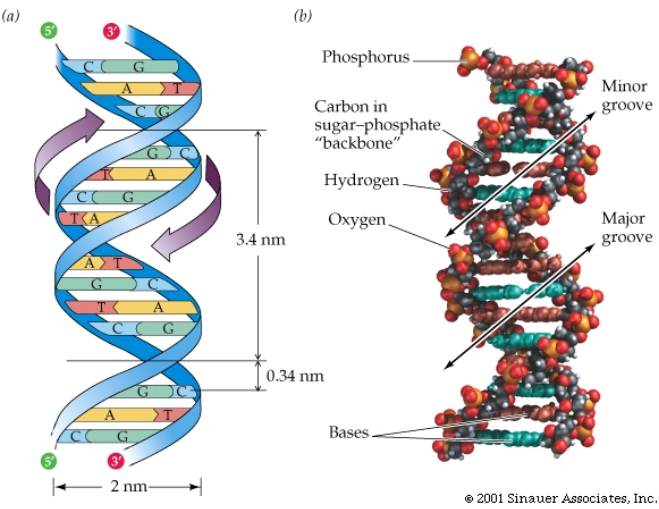
\includegraphics[width=.8\textwidth]{figures/spatial.png}
	\caption{Double stranded DNA helix.\label{o:latex_friendly_zone}}
\end{figure}

Moreover, although usually single-stranded, some RNA sequences have the ability to form a double helix. 
However, double helix RNAs are rare and do not appear to participate in some genome related processes in the eukaryotic and prokaryotic organisms.
Since circular DNA may exist in several forms including single-stranded c-DNA, intact double-stranded c-DNA (closed circles with both strands covalently linked), 
nicked ds-c-DNA (only one strand covalently linked) and in the form of “concatenated circles” their properties are not described in the attached table.

%%%%%%%%%%%%%%%%%%%%%%%%%%%%%%%%%%%%%%%%%%%%
\subsection{Eukaryotic genome organization}
%%%%%%%%%%%%%%%%%%%%%%%%%%%%%%%%%%%%%%%%%%%%
Eukaryotes are organisms whose cells have a nucleus enclosed within a nuclear envelope \cite{BioDict}.
In eukaryotic cells nucleic acid is situated in a membrane-bound organelle called the nucleus.
The nuclear genome is split into a set of linear double-helix DNA molecules, each contained in a chromosome. 
A chromosome itself is a linear string of DNA wrapped around associated proteins that give the connected nucleic acid bases a structure.

\begin{figure}[!ht]
	\centering
	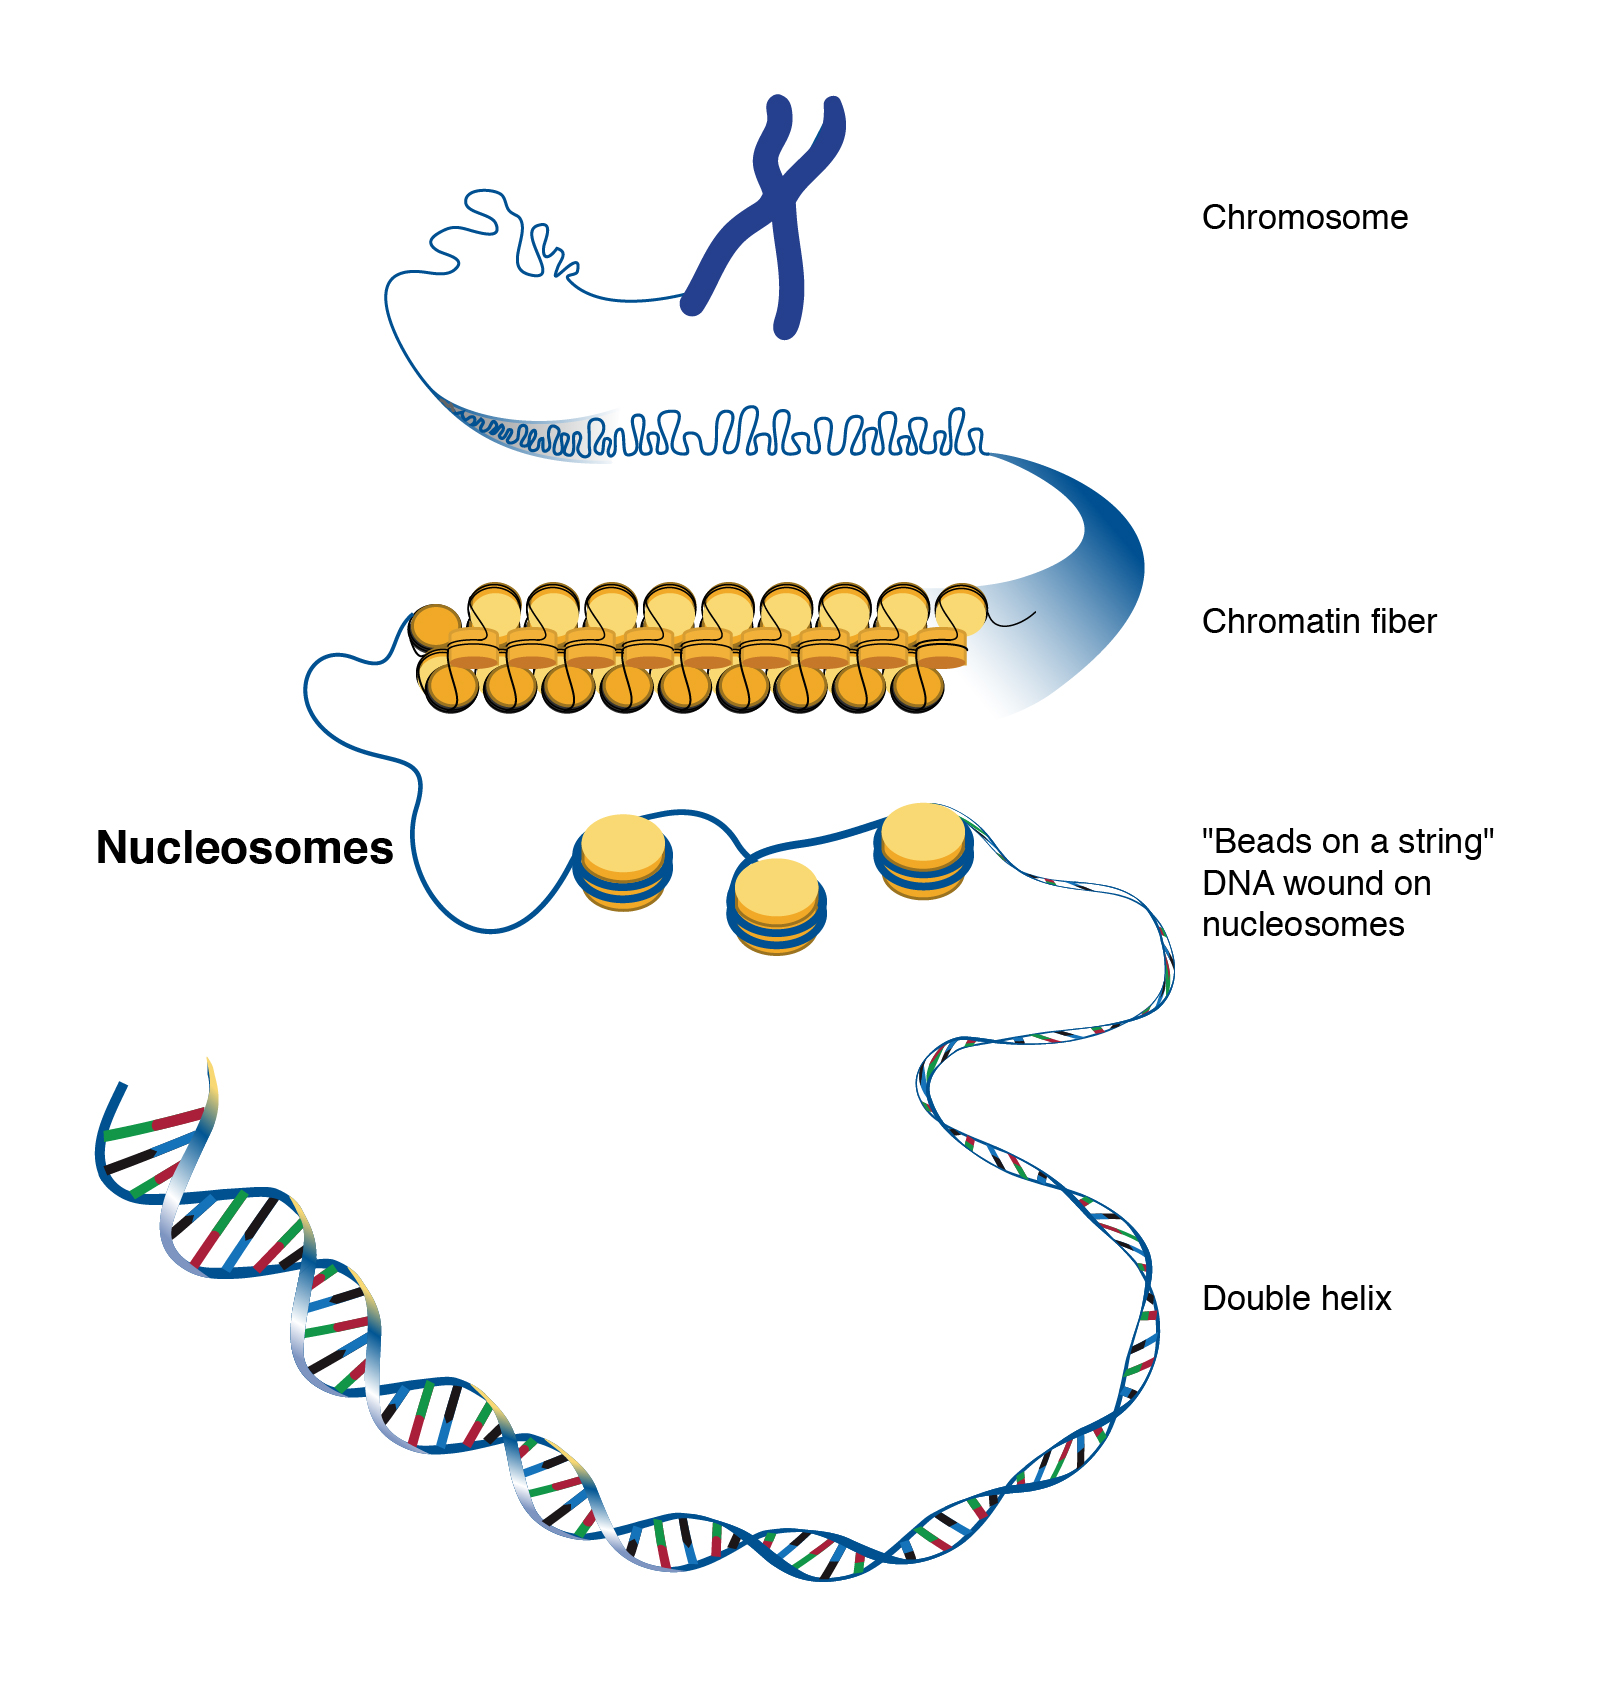
\includegraphics[width=.8\textwidth]{figures/nucleosome1}
	\caption{Eukatyotic genome organization.\label{o:latex_friendly_zone}}
\end{figure}

No exceptions to this pattern are known: eukaryotes that have been studied posess DNA molecules that are always linear and have at least two chromosomes. \cite{Genomes3}
The only variability at this level of organization of eukaryotic genome is coherent with the number of chromosomes. 
Moreover, it appears, that biological features of an organism have no dependence on the number of chromosomes. 

The ends of eukaryotic chromosomes are also the ends of linear duplex DNA and as such require a special structure to ensure that they are maintained. 
The reason for this is connected with the way in which double-stranded DNA is replicated \cite{PrinciplesOfGeneManipulation}.
In the absence of a method for completing the ends, chromosomes would become shorter after each cell division.

Telomeres are specialized nucleic acid sequences whose role is to protect the ends of chromosomes.
In most eukaryotes the telomere consists of a short repeat of TTAGGG many hundreds of units long, but the repeated segment might differ among species.
Also, these repeats vary considerably in length between species, however each species maintains a fixed average telomere length in its germline.

Despite the size of a nucleus (5-10 um), an overall length of DNA in the human cell is approximately 2.1m and can be packed inside the cell because of the method the nucleic acid is stored. 

% \begin{figure}[!ht]
% 	\centering
% 	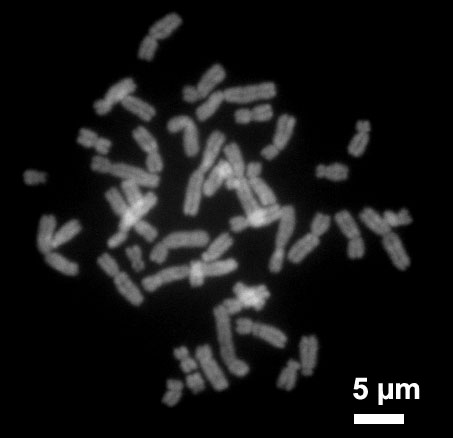
\includegraphics[width=.5\textwidth]{figures/hc.jpg}
% 	\caption{Human chromosomes during metaphase.\label{o:latex_friendly_zone}}
% \end{figure}

The genetic material in viruses and bacteria consists of strings of DNA or RNA almost devoid of proteins. 
However, in eukaryotes, a substantial quantity of protein is associated with the DNA to form chromatin. 
At the lowest level, the DNA is organized by wrapping DNA strands around he proteins called histones, that contain a large amount of positively charged amino acids arginine and lysine. 
Those amino acids, and histones in general, play the crucial structural role, making it possible to bind the negative charged phosphate groups of the DNA nucleotides.

\begin{figure}[!ht]
	\centering
	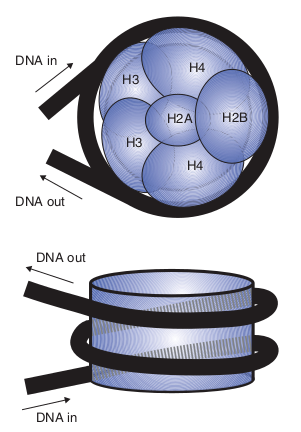
\includegraphics[width=.5\textwidth]{figures/nucleoDetailed}
	\caption{The nucleosome structure. H2A, H2B, H3 and H4 represent different types of histones. \label{o:latex_friendly_zone}}
\end{figure}

Averagely, the DNA rolled around the histones consists of 140-150 base pair, dependently on the species. 
Such a complex of DNA and histones is termed a nucleosome. 
These nucleosomes can be further coiled into increasingly larger coils up until forming chromosomes. 
However, tight coiling of DNA limits cells ability to access DNA and to process it.
Instead of being constantly coiled, the nucleic acid is usually found in a state called chromatin where some segments of acid are tightly reeled (heterochromatin), while other segments are entirely open (euchromatin). 
Euchromatin DNA is is highly accessible by the molecular complexes used by the cell and therefore is easier to manipulate with. 

The amount and extent of packing are determined by a sell, to control which sections of the genome can be expressed and which cannot. 
It affects cellular function and appears to be the predominant cause of differentiating cells type, while having the same DNA.

%%%%%%%%%%%%%%%%%%%%%%%%%%%%%%%%%%%%%%%%%%%%%
\subsection{Prokaryotic genome organization}
%%%%%%%%%%%%%%%%%%%%%%%%%%%%%%%%%%%%%%%%%%%%%
A prokaryote is a cellular organism that lacks an envelope-enclosed nucleus.
Prokaryotic genomes are very different from eukaryotic ones, in particular with regard to the physical organization of the genome within the cell.
Although the word “chromosome” is used to describe the DNA–protein structures present in prokaryotic cells, this is a misnomer as this structure does not resemble an ordinary eukaryotic chromosome.
In a typical prokaryote the genome is contained in a single, circular DNA molecule, localized within the nucleoid — the lightly staining region of the otherwise featureless prokaryotic cell.

\begin{figure}[!ht]
	\centering
	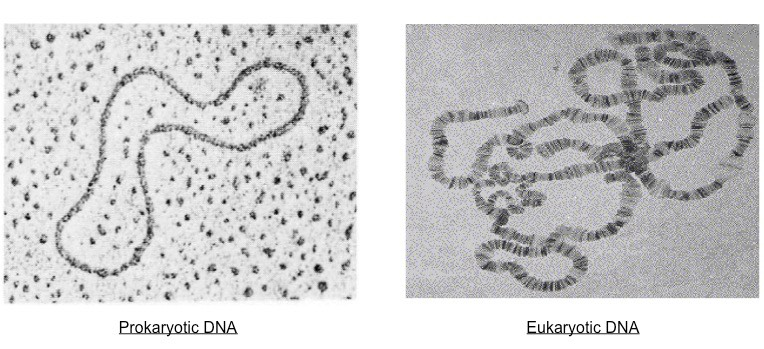
\includegraphics[width=\textwidth]{figures/pro-vs-eu-dna_med.jpeg}
	\caption{Comprasion of eukaryotic and prokaryotic DNAs \label{o:latex_friendly_zone}}
\end{figure}

Most of what is known about the organization of DNA in the nucleoid comes from studies of E. coli. 
The first feature to be recognized was that the circular E. coli genome is supercoiled. 
Supercoiling occurs when additional turns are introduced into the DNA double helix (positive supercoiling) or if turns are removed (negative supercoiling). 
With a linear molecule, the torsional stress introduced by over- or underwinding is immediately released by rotation of the ends of the DNA molecule, but a circular molecule, having no ends, cannot reduce the strain in this way. 
Instead the circular molecule responds by winding around itself to form a more compact structure. 
Supercoiling is therefore an ideal way to package a circular molecule into a small space. 
Evidence that supercoiling is involved in packaging the circular E.coli genome was first obtained in the 1970s from examination of isolated nucleoids, and subsequently confirmed as a feature of DNA in living cells in 1981. 
In E. coli, the supercoiling is thought to be generated and controlled by two enzymes, DNA gyrase and DNA topoisomerase I.

Despite the conventional prokaryotic genome structure, an increasing number of linear genomes are being found. 
Linear molecules have free ends, which must be distinguishable from DNA breaks, so these chromosomes require terminal structures equivalent to the telomeres 
of eukaryotic chromosomes. In Borrelia burgdorferi and Agrobacterium tumefaciens, the real chromosome ends are distinguishable because a covalent linkage is formed 
between the 5` and 3` ends of the polynucleotides in the DNA double helix, and in Streptomyces coelicolor the ends appear to be marked by special binding proteins.

%%%%%%%%%%%%%%%%%%%%%%%%%%%%%%%%%%%%%%%%%
\subsection{Viral genome organization}
%%%%%%%%%%%%%%%%%%%%%%%%%%%%%%%%%%%%%%%%%

To begin with, viruses are out-of-cell forms of life. It means, that their lifecycle and structure are generally less complicated comparely to others.
Viruses can be extremely simple in design, consisting of nucleic acid surrounded by a protein coat known as a capsid. The capsid is composed of smaller protein components referred to as capsomers. The capsid+genome combination is called a nucleocapsid.

\begin{figure}[!ht]
	\centering
	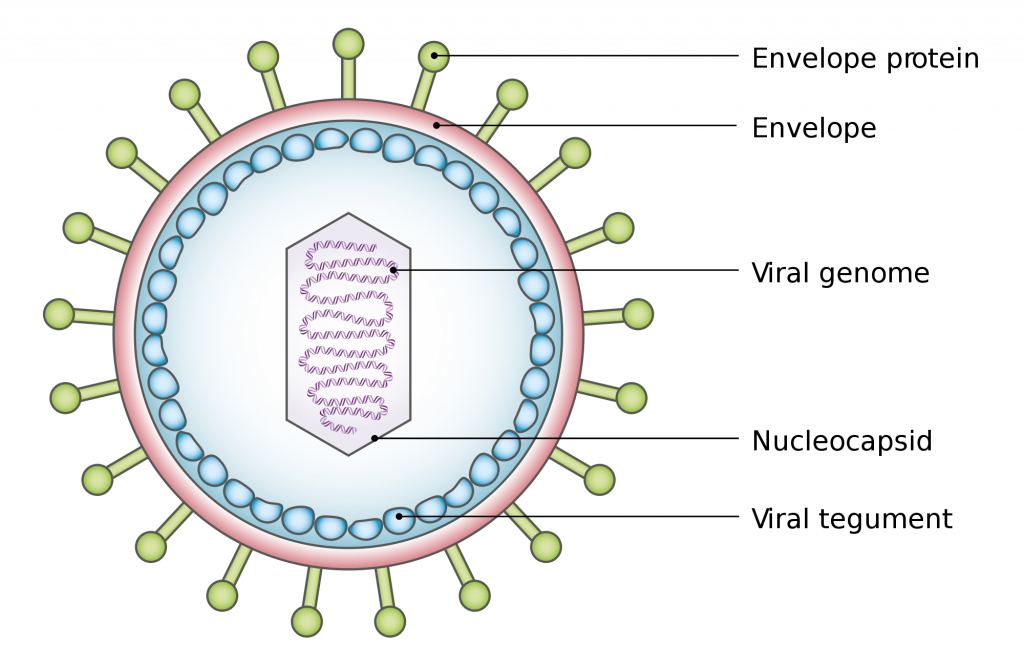
\includegraphics[width=.75\textwidth]{figures/virus.png}
	\caption{Virus Characteristics. \label{o:latex_friendly_zone}}
\end{figure}

Viruses can also possess additional components, with the most common being an additional membranous layer that surrounds the nucleocapsid, called an envelope. 
The envelope is actually acquired from the nuclear or plasma membrane of the infected host cell, and then modified with viral proteins called peplomers. 
Some viruses contain viral enzymes that are necessary for infection of a host cell and coded for within the viral genome. 
A complete virus, with all the components needed for host cell infection, is referred to as a virion.

While cells contain double-stranded DNA for their genome, viruses are not limited to this form. 
Moreover, as it was mentioned at the very beginning, apart from the dsDNA (double stranded DNA) viruses, there are also viruses with single-stranded DNA (ssDNA), double-stranded RNA (dsRNA), and single-stranded RNA (ssRNA). 
In this last category, the ssRNA can either be positive-sense (+ssRNA, meaning it can transcribe a message, like mRNA) or it can be negative-sense (-ssRNA, indicating that it is complementary to mRNA). Some viruses even start with one form of nucleic acid in the nucleocapsid and then convert it to a different form during replication.
In addition, these can be multipartite, meaning they consist of several RNA molecules.

In general, DNA viruses tend to be larger in size than RNA viruses and the single stranded genomes are smaller than those that are double-stranded. 
It is hypothesized that single-stranded virus are smaller because that type of molecule is more fragile than the double stranded molecule. 
This is generally true for both ssDNA and ssRNA viruses.
Among the double-stranded genomes, these can either have 'small' or 'large' genomes. 
One major difference between the two genomes is the mechanism of DNA replication. 
Small genomes use host polymerase activities, whereas large genomes encode an own DNA polymerase.


%%%%%%%%%%%%%%%%%%%%%%%%%%%%%%%%%%%%%%%%%%%%%%%%%%%
\subsection{Genes: location and general structure}
%%%%%%%%%%%%%%%%%%%%%%%%%%%%%%%%%%%%%%%%%%%%%%%%%%%
Gene is a sequence of nucleotides in DNA or RNA that encodes the synthesis of a gene product, either RNA or protein that have distinctive features. 
At present the nature of all of these specific features is not fully understandable, and sequence inspection is therefore not a foolproof way of locating genes\cite{Genomes3}.

Apart from the usual genes, pseudogenes are also present in different genomes.
Pseudogenes are sequences of genomic DNA with such similarity to normal genes that they are regarded as non-functional copies or close relatives of genes\cite{PrinciplesOfGeneManipulation}. 
They are formed in two ways:
\begin{itemize}
	\item Classical duplicated pseudogenes are formed when genes that are tandemly duplicated accumulate mutations such that one of the genes becomes non-functional.
	These mutations may prevent transcription and/or translation.
	\item Processed pseudogenes are formed by the accumulation of mutations in a gene that has been retrotransposed to a new location. 
	They are characterized by an absence of introns that are present in the parental gene.
\end{itemize} 

Genes that code for proteins comprise open reading frames (ORFs) consisting of a series of codons (trinucleotides) that specify the amino acid sequence of the protein that the gene codes for. 
The ORF begins with an initiation codon — usually (but not always) ATG — and ends with a termination codon: TAA, TAG, or TGA. 
Searching a DNA sequence for ORFs that begin with an ATG and end with a termination triplet is therefore one way of looking for genes. 
The analysis is complicated by the fact that each DNA sequence has six reading frames, three in one direction and three in the reverse direction on the complementary strand.

\begin{figure}[!ht]
	\centering
	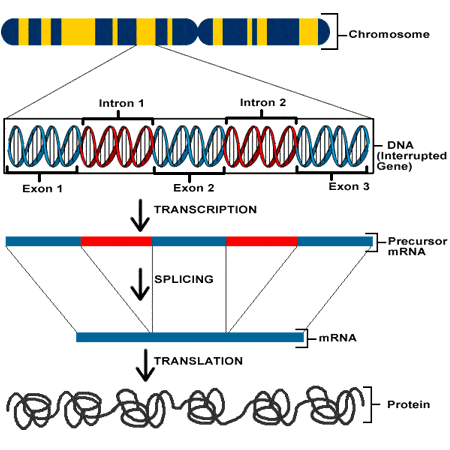
\includegraphics[width=.6\textwidth]{figures/eukaryotic_transcription_2.png}
	\caption{Intron and exon organization during DNA-coherent processes at the cell's lifecycle.\label{o:latex_friendly_zone}}
\end{figure}

The key to the success of ORF scanning is the frequency with which termination codons appear in the DNA sequence. 
If the DNA has a random sequence and a GC content of 50\% then each of the three termination codons — TAA, TAG, and TGA — will appear, on average, once every 64 bp. 
If the GC content is greater than 50\% then the termination codons, being AT – rich, will occur less frequently, but one will still be expected every 100–200 bp. 
This means that random DNA should not show many ORFs longer than 50 codons in length.
Most genes, on the other hand, are longer than 50 codons: the average lengths are 317 codons for Escherichia coli, 483 codons for Saccharomyces cerevisiae, and approximately 450 codons for humans \cite{FindingGenes}. 
ORF scanning, in its simplest form, therefore takes a figure of, say, 100 codons as the shortest length of a putative gene and records positive hits for all ORFs longer than this.

With bacterial genomes, simple ORF scanning is an effective way of locating most of the genes in a DNA sequence.
The real genes in the sequence cannot be mistaken because they are much longer than 50 codons in length. 
With bacteria the analysis is further simplified by the fact that the genes are very closely spaced and hence there is relatively little intergenic DNA in the genome (only 11\% for E. coli). 
The most of bacterial genes do not overlap.

\begin{figure}[!ht]
	\centering
	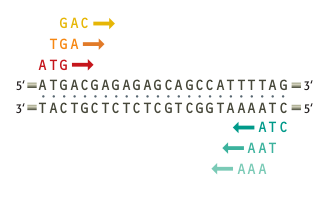
\includegraphics[width=.6\textwidth]{figures/ORF2.png}
	\caption{Both
	strands are read in the 5`3`direction. Each
	strand has three reading frames, depending
	on which nucleotide is chosen as the
	starting position.\label{o:latex_friendly_zone}}
\end{figure}

Although ORF scans work well for bacterial genomes, they are less effective for locating genes in DNA sequences from higher eukaryotes. 
This is partly because there is substantially more space between the real genes in a eukaryotic genome (for example, approximately 62\% of the human genome is intergenic), increasing the chances of finding spurious ORFs. 
But the main problem with the human genome and the genomes of higher eukaryotes in general is that their genes are often split by introns (non-coding regions of gene), and so do not appear as continuous ORFs in the DNA sequence. 
Many exons (coding regions of gene) are shorter than 100 codons, some consisting of fewer than 50 codons, and continuing the reading frame into an intron usually leads to a termination sequence that appears to close the ORF. 
In other words, the genes of a higher eukaryote do not appear in the genome sequence as long ORFs, and simple ORF scanning cannot locate them.

In addition, since some viruses (mainly eukaryotic ones) have intron-exon stuctures in their genomes \cite{Genes3}, ORF scanning is not the irrefragable method of locating genes among them.

ORF scanning is appropriate for protein-coding genes, but genes for functional RNAs such as rRNA and tRNA do not comprise open reading frames. 
Functional RNA molecules do, however, have their own distinctive features, which can be used to aid their discovery in a genome sequence. 

\begin{figure}[!ht]
	\centering
	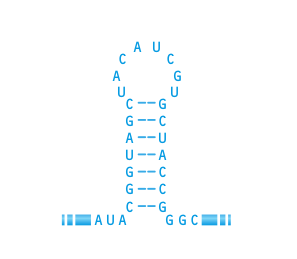
\includegraphics[width=.5\textwidth]{figures/rna.png}
	\caption{A typical RNA intramolecular base pairing
	structure.\label{o:latex_friendly_zone}}
\end{figure}

The most important of these features is the ability to fold into a secondary structure, such as the cloverleaf adopted by tRNA molecules. 
These secondary structures are held together by base pairing not between two separate polynucleotides, as in the DNA double helix, 
but between different parts of the same polynucleotide — intramolecular base pairing. 

In order for intramolecular base pairs to form, the nucleotide sequences in the two parts of the molecule must be complementary, 
and to produce a complex structure such as the cloverleaf, the components of these pairs of complementary sequences must be arranged in a characteristic order within the RNA sequence. 
These features provide a wealth of information that can be used to locate tRNA genes in a genome sequence.

As well as tRNAs, rRNAs and some of the small functional RNAs also adopt secondary structures that have sufficient complexity to enable their genes to be identified without too much difficulty \cite{rna}. 
Other functional RNA genes are less easy to locate because the RNAs take up structures that involve relatively little base pairing or the base pairing is not in a regular pattern.

%%%%%%%%%%%%%%%%%%%%%%%%%%%%%%%%%%%%%%%%%%%%%%%%%%%%%%%%%%
\section{Existing Solutions For Genome Data Representing}
%%%%%%%%%%%%%%%%%%%%%%%%%%%%%%%%%%%%%%%%%%%%%%%%%%%%%%%%%%
With the rapid development of next-generation sequencing technologies, hundreds of thousands of genomes have been sequenced. %(http://www.genomesonline.org/)
All the sequence data as well as the annotations are collected in the genome databases and are publicly available 
through web portals such as the NCBI genome portal (http://www.ncbi.nlm.nih.gov/genome/) and the EBI genome database website (http://www.ebi.ac.uk/Databases/genomes.html). 

By systematic integration of genome sequences together with annotations generated through much heterogeneous data, genome browser provides a unique platform 
for molecular biologists to browse, search, retrieve and analyze these genomic data efficiently and conveniently. 
With a graphical interface, genome browser helps users to extract and summarize information intuitively from huge amount of raw complex data. 

In general, genome browser can be divided into web-based browsers and stand-alone applications. 
Web-based genome browsers which usually are more usable in promoting biological research due to their data quality, flexible accessibility and high performance
\begin{itemize}
	\item Firstly, dedicated organizations often collect and integrate high-quality annotation data into web-based genome browsers, providing plentiful up-to-date information for the community. 
	\item Secondly, users can access them anywhere with a standard web browser, avoiding any additional effort of setting up local environment for application installation and data preparation. 
	\item Thirdly, web-based genome browsers are usually installed on high performance servers and can support more complex and larger scale data types and applications. 
\end{itemize}

%%%%%%%%%%%%%%%%%%%%%%%%%%%%%%%%%%%%%%%
\subsection{Web-based genome browsers}
%%%%%%%%%%%%%%%%%%%%%%%%%%%%%%%%%%%%%%%

Currently, there are two types of web-based genome browsers. 

The first type is the multiple-species genome browsers such as the Ensembl project \cite{ENSEMBLgb}, the UCSC genome database \cite{UCSCgb} and the NCBI Map viewer website \cite{NCBIgb}.
These genome browsers promote cross-species comparative analysis. 
Most of them contain abundant annotations, covering gene model, transcript evidence, expression profiles, regulatory data, genomic conversation, etc. 
Each set of pre-computed annotation data is called a track in genome browsers. 
The essence of a genome browser is to pile up multiple tracks under the same genomic coordinate along the Y-axis, thus users could easily examine the consistency or difference of the annotation data and make their judgments of the features of the genomic region.

The other type is the species-specific genome browsers which mainly focus on one model organism and may have more annotations for a particular species. 
Powered by the Generic Model Organism Database (GMOD) project (http://gmod.org/), dozens of open-source software tools are collected for creating and managing genome biological databases.
The GBrowse framework \cite{GBrowse} is one of the most popular tools in the GMOD project. 
Table 2 lists several mainstream web-based genome browsers, including Ensembl, the UCSC genome browser and the GBrowse, which are accessed by a large number of users worldwide.

%%%%%%%%%%%%%%%%%%%%%%%%%%%%%%%%%%%%%%%%%%
\subsection{Functionalities and features}
%%%%%%%%%%%%%%%%%%%%%%%%%%%%%%%%%%%%%%%%%%

A web-based genome browser often provides a centralized or a set of databases to store different types of annotation data obtained from several organizations. 
The challenge for the general genome browsers is how to display this information properly for different genomic scales. 
Massive amounts of information need to be incorporated into the picture when a large genomic area is requested, which could overburden the server and the network. 
Furthermore, too many heavy and complicated details also disturb the user attention. 

\begin{figure}[!ht]
	\centering
	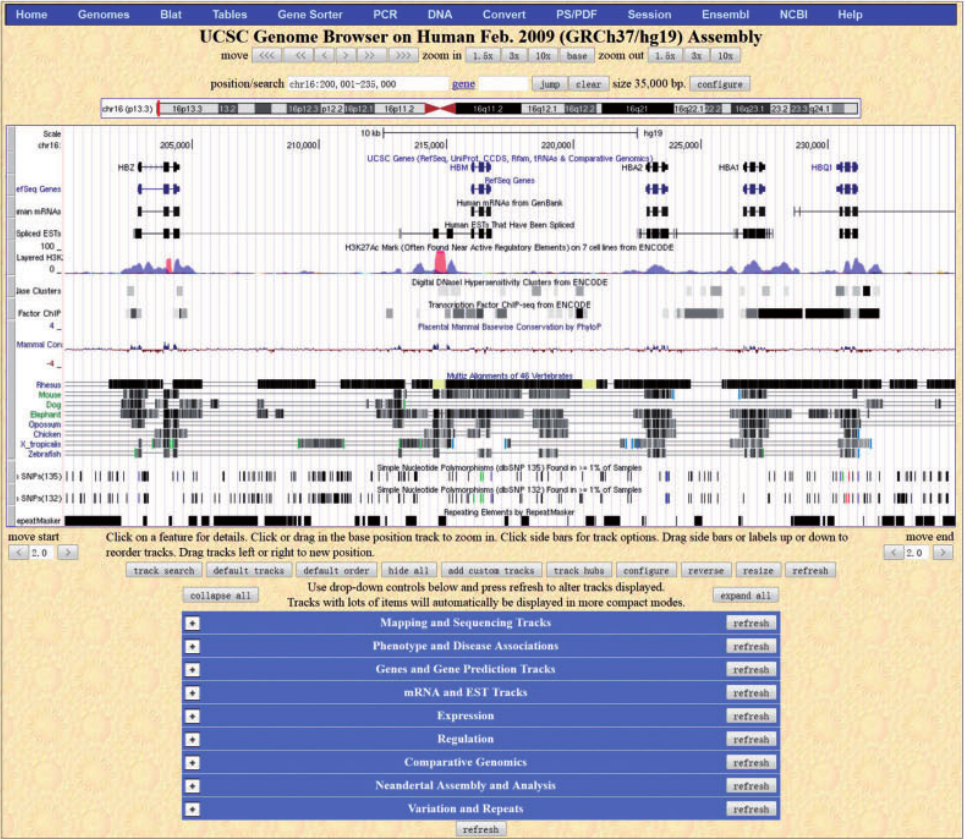
\includegraphics[width=.9\textwidth]{figures/ucsc_gb.png}
	\caption{The main user interface of the UCSC genome browser showing the default tracks in default order for the human alpha-globin gene cluster.\label{o:latex_friendly_zone}}
\end{figure}

Being the one of the big players in genomic data visualization, The UCSC genome browser tries to solve the problem by providing multiple views for a track [5]. 
Every track can be viewed in different modes such as dense, or fully expanded or can be hidden. 
The user can go deeper on the dense track 25 to open it in full mode. 
There are many scales possible for the track display. 
The lowest is a single chromosome and the highest scale is the sequence of base pairs.
The dense view of some tracks could be displayed to hide complicated details when zooming out to a large area of a chromosome, so that the user has a broad picture of the selected chromosome region.

\begin{figure}[!ht]
	\centering
	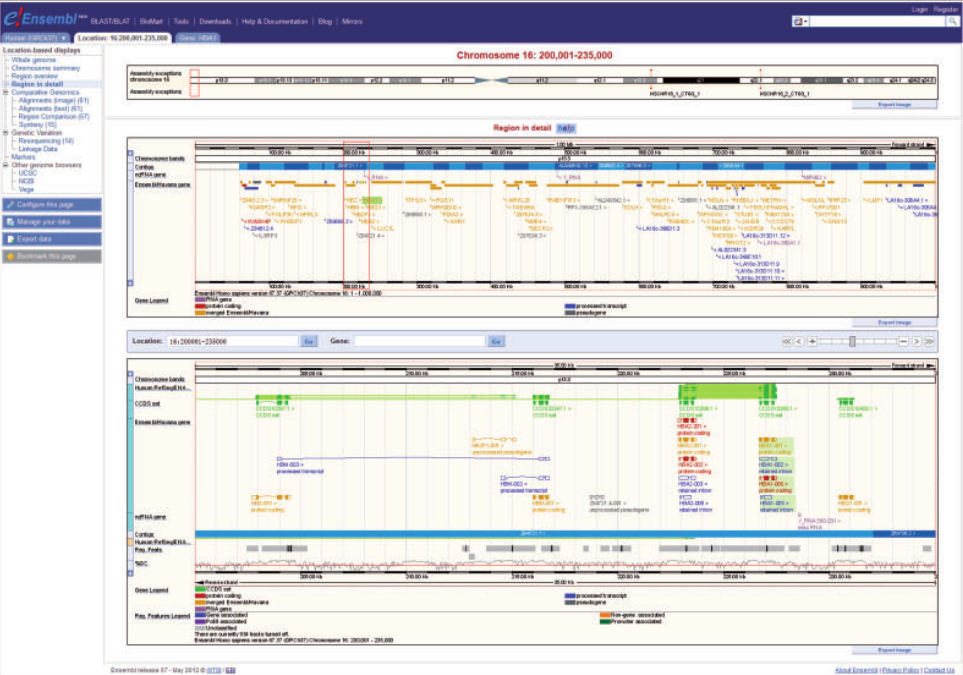
\includegraphics[width=.9\textwidth]{figures/ensembl_gb.png}
	\caption{The user interface of the Ensembl genome browser with default setting of the annotation tracks, showing the alpha-globin gene cluster. The graphical annotations are displayed in the main
	body divided in three sections from top to bottom.\label{o:latex_friendly_zone}}
\end{figure}

The Ensembl genome browser provides the same user interface for each organism. 
The main body of the interface contains two panels. 
The left panel lists the main menu for location-based displays at different levels from whole genome, chromosome summary to region overview and region in detail. 
And links to comparative genomics, genetic variation as well as sequence markers are also provided. 
The main panel is arranged in three sections from top to bottom, providing different scales for users to analyze the genome.
In addition to the location view, Ensembl provides separate pages to display various types of information, organized in a tabbed structure.

It is useful to have an overview of a large area of the chromosome and look into several small regions for details simultaneously. 
Putting paralogous genes together in one page could promote comparative analysis greatly. 
For example, NCBI sequence viewer supports users to view different regions inside the same chromosome, providing flexible multiple-panel-based navigating approach with different color cursors indicating the corresponding genomic locations.
Meanwhile, ABrowse supports users to visualize multiple genome regions of different chromosomes/genomes in separated in-page windows [11], while the separated windows are not fully operable as the main browsing canvas.

As was mentioned above, there are species-specific genome browsers are available online.
The bright examples of such tools are the MSU rice genome browser and the Rice-Map genome browser \cite{RMgb}.

\begin{table}[]

	\caption{Main functions of the mainstream genome browsers.}\label{t:1}
	\smallskip
	\centering

	\begin{tabular}{|l|l|l|c|}
	\hline
	\multicolumn{1}{|c|}{\textbf{Features}}                              & \multicolumn{1}{c|}{\textbf{UCSC}}                                               & \multicolumn{1}{c|}{\textbf{Ensemble}}                                                            & \textbf{GBrowse}                                                                                           \\ \hline
	\multicolumn{4}{|c|}{Visualization}                                                                                                                                                                                                                                                                                                                                      \\ \hline
	\begin{tabular}[c]{@{}l@{}}Annotation \\ navigation\end{tabular}     & \begin{tabular}[c]{@{}l@{}}Page-based browsing,\\ enabling dragging\end{tabular} & \begin{tabular}[c]{@{}l@{}}Page-based\\ browsing\end{tabular}                                     & \multicolumn{1}{l|}{\begin{tabular}[c]{@{}l@{}}Map-like browsing\\ within a limited\\ region\end{tabular}} \\ \hline
	\begin{tabular}[c]{@{}l@{}}Multiple in-page\\ windows\end{tabular}   & \multicolumn{1}{c|}{-}                                                           & \multicolumn{1}{c|}{-}                                                                            & -                                                                                                          \\ \hline
	\multicolumn{4}{|c|}{Data retrieval and analysis}                                                                                                                                                                                                                                                                                                                        \\ \hline
	Query system                                                         & Table Browser                                                                    & BioMart                                                                                           & -                                                                                                          \\ \hline
	\begin{tabular}[c]{@{}l@{}}User-oriented \\ analysis\end{tabular}    & \begin{tabular}[c]{@{}l@{}}Direct data \\ submission\end{tabular}                & \multicolumn{1}{c|}{-}                                                                            & \multicolumn{1}{l|}{Plugin tools}                                                                          \\ \hline
	\begin{tabular}[c]{@{}l@{}}Machine-oriented\\ interface\end{tabular} & \multicolumn{1}{c|}{-}                                                           & \begin{tabular}[c]{@{}l@{}}Through\\ BioMart\end{tabular}                                         & \multicolumn{1}{l|}{Through BioDAS}                                                                        \\ \hline
	\multicolumn{4}{|c|}{Customization}                                                                                                                                                                                                                                                                                                                                      \\ \hline
	Upload user tracks                                                   & \multicolumn{1}{c|}{+}                                                           & \multicolumn{1}{c|}{+}                                                                            & +                                                                                                          \\ \hline
	\begin{tabular}[c]{@{}l@{}}User-contributed\\ contents\end{tabular}  & \begin{tabular}[c]{@{}l@{}}Session-based\\ data restoring\end{tabular}           & \begin{tabular}[c]{@{}l@{}}Personal\\ annotation,\\ bookmark\\ and group\\ mechanism\end{tabular} & -                                                                                                          \\ \hline
	\end{tabular}
\end{table}

In the MSU rice genome browser, users can search the OsSPL14 gene by specifying ‘SPL14’ in the search box.
Powered by the GBrowse platform, the MSU rice genome browser provides annotation views with different scales, including chromosome overview, regional view and detailed view. 
The large-scale view provides a broader picture for users to inspect the upstream and downstream annotation conveniently. 
In the detailed annotation canvas, more than 82 annotation tracks are provided, covering gene model, transcript evidence, expression profiling, sequence alignment, genetic marker, SNP, RNA-Seq coverage and other genomic features. 
In addition to the basic gene model information, users may inspect this gene in different development stages through various RNA-Seq expression data. 

\begin{figure}[!ht]
	\centering
	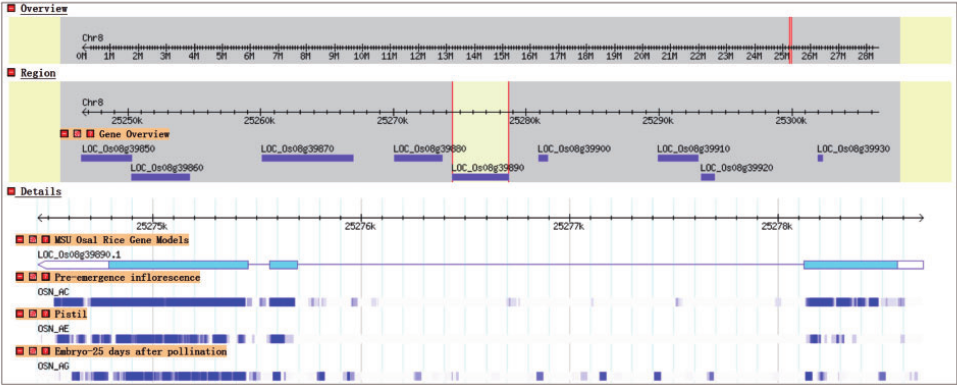
\includegraphics[width=.9\textwidth]{figures/ss-1.png}
	\caption{The user interface of the MSU rice genome browser. The chromosome overview is displayed at the top, the regional view is shown at the middle and the bottom section is the detailed view for four annotation tracks.\label{o:latex_friendly_zone}}
\end{figure}

In the Rice-Map genome browser different annotation tracks are organized in a map-like visualization canvas, with the name of opened tracks listed in the right panel. 
Besides basic gene annotation, there are rich annotation for cross genome alignments and conservation values, offering important clues to investigate this gene in other plants.

\begin{figure}[!ht]
	\centering
	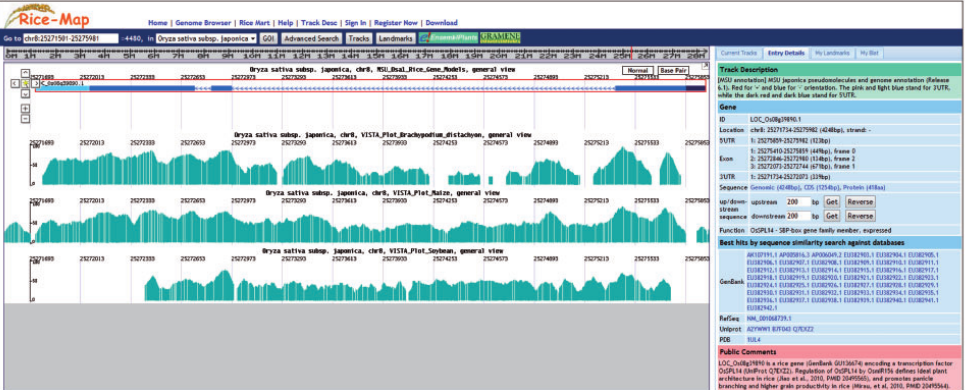
\includegraphics[width=.9\textwidth]{figures/ss-2.png}
	\caption{The Rice-Map genome browser. The detailed information for individual entries is shown in the right panel, interpreting the data resource, entry location, sequence and function etc.\label{o:latex_friendly_zone}}
\end{figure}

Since genome browsers are capable of providing the user with a plenty of different biology-specific information, the definitions of those terms are not provided by this thesis.